\documentclass[default, sn-standardnature]{sn-jnl}% Default with double column layout

%%%% Standard Packages
%%<additional latex packages if required can be included here>
%%%%

%%%%%=============================================================================%%%%
%%%%  Remarks: This template is provided to aid authors with the preparation
%%%%  of original research articles intended for submission to journals published
%%%%  by Springer Nature. The guidance has been prepared in partnership with
%%%%  production teams to conform to Springer Nature technical requirements.
%%%%  Editorial and presentation requirements differ among journal portfolios and
%%%%  research disciplines. You may find sections in this template are irrelevant
%%%%  to your work and are empowered to omit any such section if allowed by the
%%%%  journal you intend to submit to. The submission guidelines and policies
%%%%  of the journal take precedence. A detailed User Manual is available in the
%%%%  template package for technical guidance.
%%%%%=============================================================================%%%%

\jyear{2022}%
\newgeometry{left=2cm, right=2cm}
\linespread{1.5}

%% as per the requirement new theorem styles can be included as shown below
\theoremstyle{thmstyleone}%
\newtheorem{theorem}{Theorem}%  meant for continuous numbers
%%\newtheorem{theorem}{Theorem}[section]% meant for sectionwise numbers
%% optional argument [theorem] produces theorem numbering sequence instead of independent numbers for Proposition
\newtheorem{proposition}[theorem]{Proposition}%
%%\newtheorem{proposition}{Proposition}% to get separate numbers for theorem and proposition etc.

\theoremstyle{thmstyletwo}%
\newtheorem{example}{Example}%
\newtheorem{remark}{Remark}%

\theoremstyle{thmstylethree}%
\newtheorem{definition}{Definition}%
% \usepackage{tikz}
% \newcommand*{\circled}[1]{\lower.7ex\hbox{\tikz\draw (0pt, 0pt)%
%     circle (.5em) node {\makebox[1em][c]{\small #1}};}}
\raggedbottom
%%\unnumbered% uncomment this for unnumbered level heads
%! path of figs

\graphicspath{{/Users/songshgeo/Documents/Pycharm/WGRegimes_YRB_2020/figures/}}
\begin{document}

\title{Supporting Materials of ``Identifying regime transitions for water governance at a basin scale''}

%%=============================================================%%
%% Prefix	-> \pfx{Dr}
%% GivenName	-> \fnm{Joergen W.}
%% Particle	-> \spfx{van der} -> surname prefix
%% FamilyName	-> \sur{Ploeg}
%% Suffix	-> \sfx{IV}
%% NatureName	-> \tanm{Poet Laureate} -> Title after name
%% Degrees	-> \dgr{MSc, PhD}
%% \author*[1,2]{\pfx{Dr} \fnm{Joergen W.} \spfx{van der} \sur{Ploeg} \sfx{IV} \tanm{Poet Laureate}
%%                 \dgr{MSc, PhD}}\email{iauthor@gmail.com}
%%=============================================================%%

\author[1]{\fnm{Shuang} \sur{Song}}\email{songshgeo@mail.bnu.edu.cn}

\author[1]{\fnm{Shuai} \sur{Wang}}\email{shuaiwang@bnu.edu.cn}
% \equalcont{These authors contributed equally to this work.}

\author[1]{\fnm{Xutong} \sur{Wu}}\email{wuxutong@bnu.edu.cn}
% \equalcont{These authors contributed equally to this work.}
\author[2]{\fnm{Yongping} \sur{Wei}}\email{yongping.wei@uq.edu.au}
\author[3]{\fnm{Graeme S.} \sur{Cumming}}\email{graeme.cumming@jcu.edu.au}
\author[4]{\fnm{Yue} \sur{Qin}}\email{qinyue@pku.edu.cn}
\author[5]{\fnm{Xilin} \sur{Wu}}\email{wuxilin20@mails.ucas.ac.cn}
\author*[1,5]{\fnm{Bojie} \sur{Fu}}\email{bfu@rcees.ac.cn}

\affil*[1]{\orgdiv{State Key Laboratory of Earth Surface Processes and Resource Ecology}, \orgname{Beijing Normal University,}, \orgaddress{\city{Beijing}, \postcode{100875}, \state{Beijing}, \country{China}}}

\affil[2]{\orgdiv{School of Earth and Environmental Sciences}, \orgname{The University of Queensland}, \orgaddress{\city{Brisbane}, \postcode{4067}, \state{QLD}, \country{Australia}}}

\affil[3]{\orgdiv{ARC Centre of Excellence for Coral Reef Studies}, \orgname{James Cook University}, \orgaddress{\city{Townsville}, \postcode{4811}, \state{QLD}, \country{Australia}}}

\affil[4]{\orgdiv{College of Environmental Sciences and Engineering} \orgname{Peking University}, \orgaddress{\city{Beijing}, \postcode{100875}, \state{Beijing}, \country{China}}}

\affil[5]{\orgdiv{State Key Laboratory of Urban and Regional Ecology, Research Center for Eco-Environmental Sciences}, \orgname{Chinese Academy of Sciences}, \orgaddress{\city{Beijing}, \postcode{100875}, \state{Beijing}, \country{China}}}
%%==================================%%
%% sample for unstructured abstract %%
%%==================================%%

%% Comment out or remove this line before generating final copy for submission; this will also remove the warning re: "Consecutive odd pages found".
% \instructionspage

\maketitle

%% Adds the main heading for the SI text. Comment out this line if you do not have any supporting information text

\section{YRB Regions}\label{secA1}
We divide the YRB into four regions to calculate the indicators considering both socio-economic and natural conditions. The division aligns with the customary schema from publications and the YRCC~\cite{yellowriverconservancycommission2013,wang2019c,wang2016e}, so four important hydrological stations can distinguish the regions (see Figure~\ref{fig:YRB}).

\begin{itemize}
    \item \textbf{Source Region (SR):} Over 50\% of natural runoff originates from this region. The most ecological function here is water yield, as sparsely populated and less economically developed.
    \item \textbf{Upper Region (UR):} With the highest per capita irrigated land area, there are numbers of large irrigation lands in this region. However, irrigation efficiency is relatively much lower than its lower reaches.
    \item \textbf{Middle Region (MR):} Crossing Loess Plateau, a famous rich-sand area, Yellow River loads most of its sediments here with the highest soil erosion risk. The ``grain for the green'' project changed the water utilization here strikingly to reverse this situation~\cite{wu2020a}.
    \item \textbf{Lower Region (LR):} With a dense population and the traditional agricultural trajectory, the lower region used to be the largest water use region. However, as the industrial transformation going, the proportion of agriculture keeps decreasing, but LR is still the largest water use region in each aspect.
\end{itemize}

% 补充图片1:研究区示意图
\begin{figure*}[hbtp!]
    \centering
    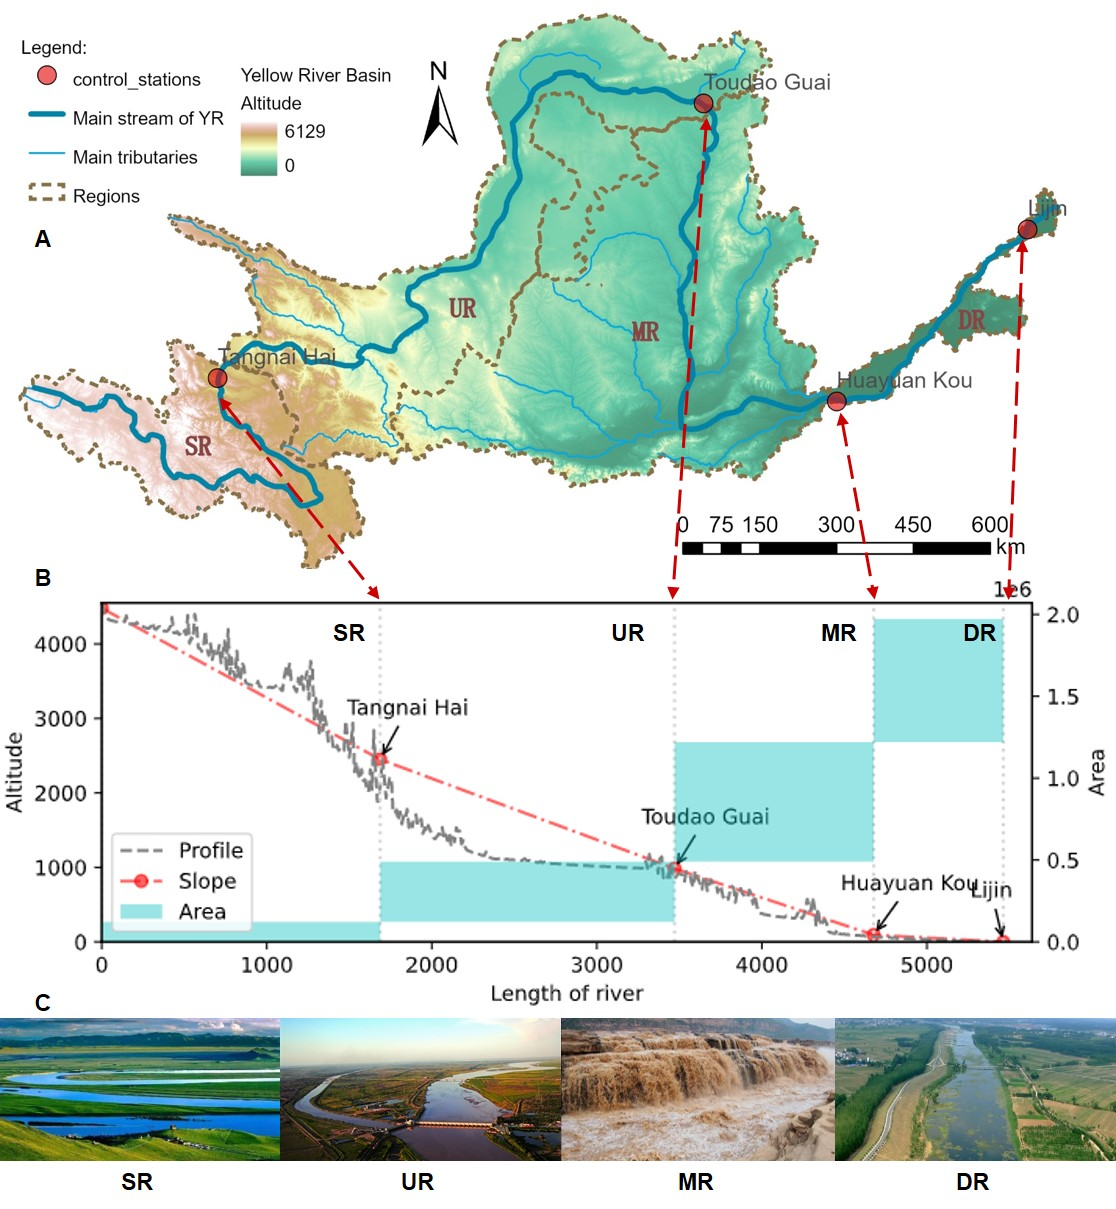
\includegraphics[width=0.6\textwidth]{sup/s1_study_area.jpg}
    \caption{
        The study area.
        \textbf{A.} Diagram of the YRB and the subdivision of the basin (SR: Source Region, UR: Upper Region, MR: Middle Region, DR: Downstream region).
        \textbf{B.} Profile of the main channel of the Yellow River. The hydrological stations control the SR, UR, MR and DR.
        \textbf{C.} Typical landscapes in different regions in the YRB.
    }\label{fig:YRB}
\end{figure*}

% % 补充图片4:天然水资源量
% \begin{figure*}[tb]
%     \centering
%     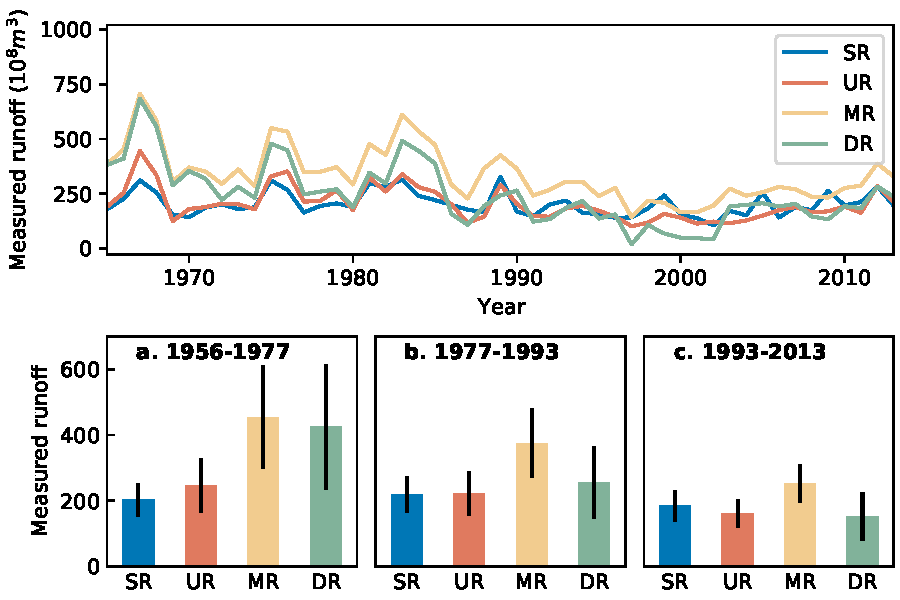
\includegraphics[width=0.8\textwidth]{sup/sf_measured_runoff.pdf}
%     \caption{Water resources in different regions.
%         \textbf{A,} changing trend of measured runoff,
%         \textbf{B, C and D} average measured runoff within different periods.
%         \textbf{E, F and G} average total water consumptions within different periods.
%     }
%     \label{fig:water resources}
% \end{figure*}


\section{SFV-index}\label{secA2}
By taking water flexibility and variability into account, the scarcity-flexibility-variability (SFV) index focus more on dynamic responses to water resources in a developing perspective, which is a valid metric of temporal changes in water stresses \cite{qin2019}. To apply this method, we need to combine three metrics following:

First, for scarcity, $A_{i, j}$ is the total water consumption as a proportion of regional multi-year average runoff volume in year $j$ and region $i$ (in this study, four regions in the YRB, \\textit{Supporting Information}~\ref{secA1}):
\begin{equation}
    A_{i, j} = \frac{WU_{i,j}}{R_{i, avg}}
\end{equation}

Second, for flexibility, $B_{i, j}$ is the inflexible water use $WU_{inflexible}$ (i.e. for thermal power plants or humans and livestock) as a proportion of average multi-year runoff, in year $i$ and region $j$:
\begin{equation}
    B_{i, j} = \frac{WU_{i, j, inflexible}}{R_{i, avg}}
\end{equation}

Finally for variability, the capacity of the reservoir and the positive effects of storage on natural runoff fluctuations are also considered.
\begin{gather}
C_i = C1_i * (1 - C2_i) \\
C1_{i, j} = \frac{R_{i, std}}{R_{i, avg}} \\
C2_{i} = \frac{RC_{i}}{R_{i, avg}}, \ if RC < R_{i, avg} \\
C2_{i} = 1, \ if RC >= R_{i, avg}
\end{gather}

In all the equations above, $R_{i, avg}$ is the average runoff in region $i$, $RC_i$ is the total storage capacities of reservoirs in the region $i$, $R_{i, std}$ is the standard deviation of runoff in the region $i$.

Finally, assuming three metrics (scarcity, flexibility and variability) have the same weights, we can calculate the $SFV$ index after normalizing them:
\begin{gather}
    V = \frac{A_{normalize} + B_{normalize} + C_{normalize}}{3}\\
    a = \frac{1}{V_{max} - V_{min}};\\
    b = \frac{1}{V_{min} - V_{max}} * V_{min}\\
    SFV = a * V + b
\end{gather}



% \begin{figure}[tb!]
% 	\centering
% 	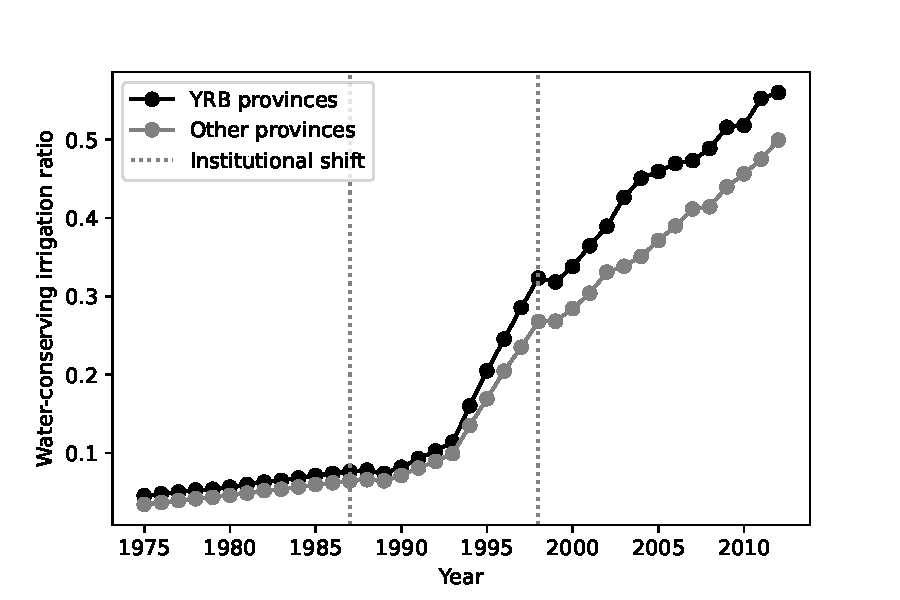
\includegraphics[width=0.9\linewidth]{sup/S3_wci.pdf}
% 	\caption{
% 	    Ratio of irrigated areas with water-saving equipments.
% 	}
% 	\label{fig:wci}
% \end{figure}


\begin{figure}[tb]
    \centering
    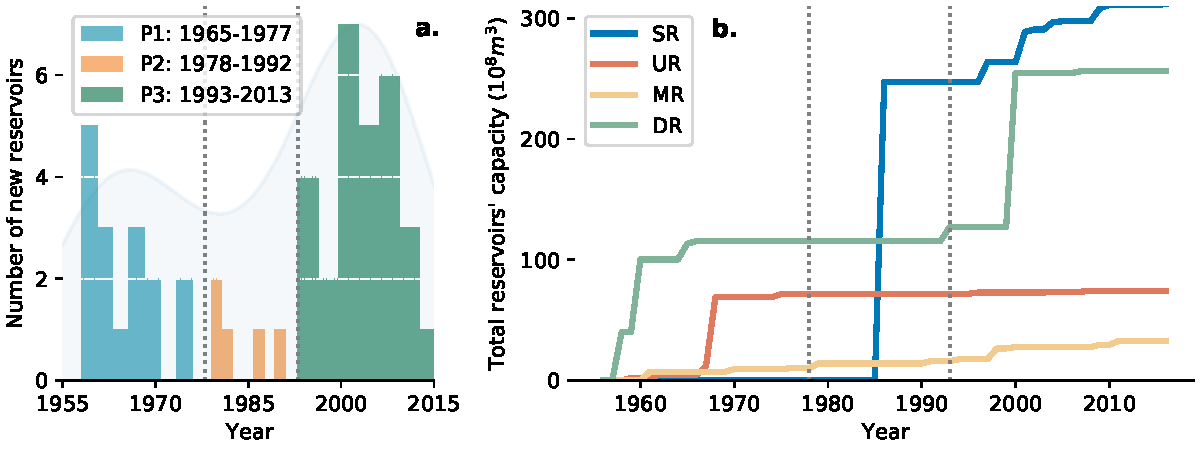
\includegraphics[width=0.6\linewidth]{sup/reservoirs.pdf}
    \caption{
        Numbers of new reservoirs in each year.
    }
    \label{fig:reservoirs}
\end{figure}

\begin{figure}
    \centering
    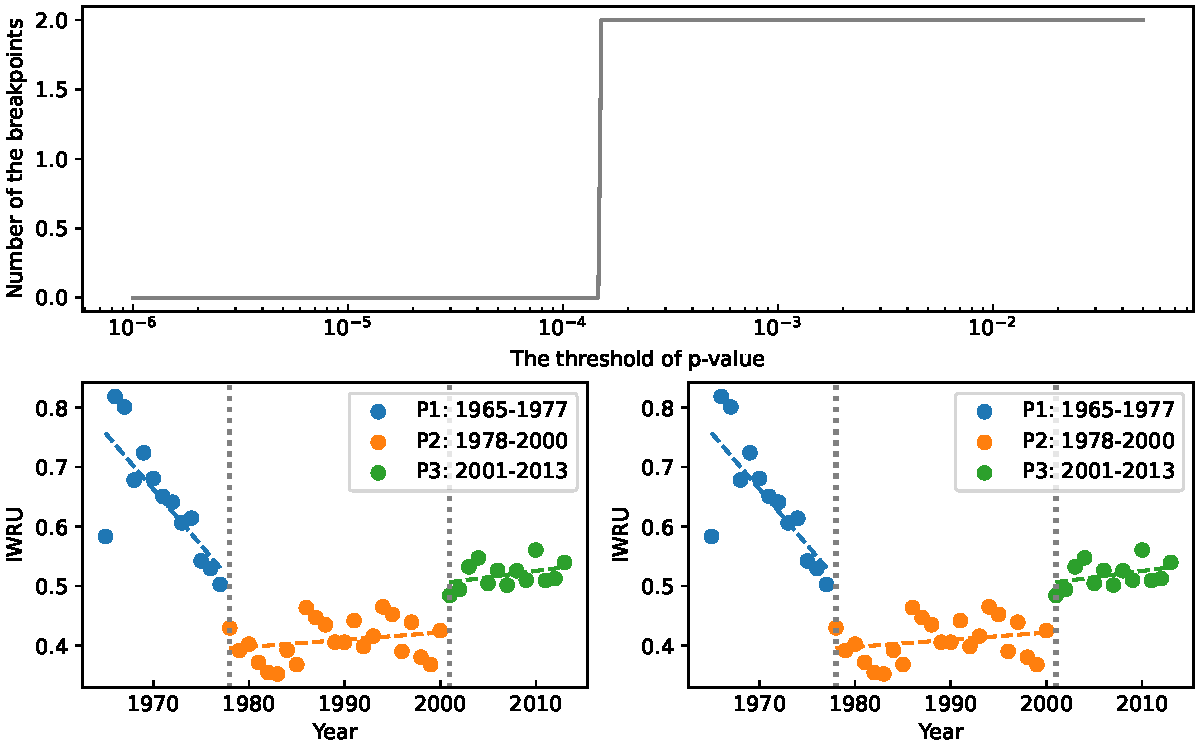
\includegraphics[width=\linewidth]{sup/sensitivity.pdf}
    \caption{
        Sensitivity analysis of the threshold of p-values.
        \textbf{A.} number of breakpoints in different p-values, the scheme with two-breakpoints are the dominant situation.
        \textbf{B.} Threshold of p-values $\alpha=0.0005$.
        \textbf{C.} Threshold of p-values $\alpha=0.05$.
    }
    \label{fig:sensitivity}
\end{figure}


\section{Datasets}\label{secA3}
\subsection*{Descriptions}
This study used multiple types of data (see Table~\ref{tab:datasets}): statistical datasets, hydrological datasets, and political datasets.

\subsubsection*{Statistical datasets}
% We used GDP data; water resources uses data extracted from the 2nd National Water Resources Assessment Program \cite{zhou2020} and statistical yearbooks \url{http://www.yrcc.gov.cn/other/hhgb/}.
The water resources use dataset was published by Zhou et al. \cite{zhou2020}, which records water utilization in different sectors along with social-economic situations at the Prefectures level. 2nd National Water Resources Assessment Program mainly extracted this dataset launched in 2002, led by the National Development and Reform Commission and the Ministry of Water Resources (see ref (1) and \url{http://www.mwr.gov.cn/english/publs/} for more details). Since then, the statistics from the survey using the same criteria have been supplemented and harmonized with the 2013 administrative divisions.

The data covers a total of subcategories of water use under four broad categories: agriculture (IRR), industry (IND), urban (URB) and rural (RUR) water use (see Zhou et al., for details \cite{zhou2020}).
% There is uncertainty at the county scale for each disaggregated water use sector, but because the corrected data has been for statistical information using the water balance method, the data are adequate for the regional scale used in this study.

\subsubsection*{Hydrological datasets}
The reservoir dataset was collected by Wang et al. \cite{wang2019c}, which introduced includes the significant new reservoirs built in the YRB since 1949 (Figure~\ref{fig:reservoirs}). YRCC labelled the regulation-oriented reservoirs among them, see \url{http://www.yrcc.gov.cn/hhyl/sngc/}). In addition, annual runoff data derived from hydrological station measurements are the same as the datasets used in \cite{wang2019c} and \cite{wang2016e}.

\subsubsection*{Political datasets}
The policy dataset collects laws and policies listed in the book \cite{yellowriverconservancycommission2013}, which are related to the Yellow River basin promulgated and implemented by departments at (such as YRCC) and above (such as national institutions) at the Basin's level (Table~\ref{tab:policies}).
In addition, some are difficult to categorize; not a landmark, but numerous water governance practices in the YRB had been recorded in ``Yellow River Events'' by the YRCC; we collected them from \url{http://www.yrcc.gov.cn/hhyl/hhjs/}.

\subsection*{Methods S3. Harmonization}
Due to the wide sources of our data set and the different spatial scales, we need to harmonize them into a practical scale.
\begin{itemize}
    \item 1. Datasets at watersheds scales:
        We directly divided the annual hydrological data and measured runoff data according to their watersheds' corresponding hydrological stations (see Figure~\ref{fig:YRB} A and B).
    \item 2. Prefecture:
        We calculate the area of each prefecture to determine whether they belong to a region, with the threshold of $95\%$:

        \begin{equation}
            S_{ij} = MAX(S_ij / S_i)
        \end{equation}

        Where $i$ refers to a specific prefecture and $j$ refers to a region within YRB, i.e. SR, UR, MR, or DR. $S_i$ refers to the area of perfect $i$, and $S_{ij}$ refers intersecting area between perfect $i$ and region $j$.
        We define perfecture $i$ belongs to region $j$ if their intersecting area $S_{ij}$ over 95\% of $S_i$, i.e.:

        \begin{equation}
            MAX(S_{ij}) > 0.95 * S_i
        \end{equation}
    \item 3. Province:
        According to the major provinces contained in different regions, we determine which region the data of that province is merged into by referring to the traditional division practice:
    \begin{itemize}
        \item SR: Qinghai Gansu and Sichuan,
        \item UR: Ningxia and Inner Mongolia,
        \item MR: Shanxi and Shaanxi,
        \item DR: Shandong, Hebei and Henan.
    \end{itemize}
\end{itemize}

Finally, when we process the location data (i.e., the location data of the reservoirs), we judge the province it belongs to according to its location and then fit it to the regional scale.

\begin{table*}[!htbp]
    \begin{center}
    \small
    \begin{minipage}{\linewidth}
    \caption{Used datasets and their sources.}\label{tab:datasets}%
    \resizebox{\linewidth}{!}{
    \begin{tabular}{lrrrp{0.4\linewidth}}
    \toprule
    Dataset & Type & Spatial scale & Time scale & Source \\
    \midrule
    1. Administrative water use & Statistical & Prefectures & 1965-2013 & 2nd National Water Resources Assessment Program \cite{zhou2020}\\
    2. GDP & Statistical & Province & 1949-2019 & Wind database \\
    3. Streamflow withdrawals & Statistical & Watershed & 2003-2019 & Yearbooks \url{http://www.yrcc.gov.cn/other/hhgb/} \\
    4. Reservoirs & Hydrological & Location & 1949-2015 & Publication \cite{wang2019c} \\
    5. Measured runoff & Hydrological & Location & 1949-2019 & Measured data \cite{wang2019c,wang2016e} \\
    6. Laws & Political & Documents & 1949-2013 & YRCC \cite{yellowriverconservancycommission2013} \\
    7. History of YRCC & Political & Documents & 1949-2002 & YRCC \cite{yellowriverarchives2004} \\
    8. YRB Events & Political & Documents & 1949-2015 & YRCC: \url{http://www.yrcc.gov.cn/hhyl/hhjs/} \\
    \botrule
    \end{tabular}}
    \end{minipage}
    \end{center}
    \end{table*}

    %% 表格
\begin{table*}
    \centering
    \small
    \caption{Policies and regulations above YRB level which affected the whole basin in water utilization}\label{tab:policies}
    \begin{minipage}{\linewidth}
    \resizebox{\linewidth}{!}{
    \begin{tabular}{p{0.6\linewidth}rp{0.35\linewidth}}
        Name & Year & Agency \\
        \midrule
        1. Water Law of PRC & 1988 & National People's Congress of the PRC \\
        2. Water Law of PRC -revised 1 & 2009 & National People's Congress of the PRC \\
        3. Water Law of PRC -revised 2 & 2016 & National People's Congress of the PRC \\
        4. Regulations on the Administration of Water Drawing Licences and The Collection of water resource fees & 2006 & State Council of the PRC \\
        5. Regulations on the Administration of Water Drawing Licences and The Collection of water resource fees -revised 1 & 2017 & State Council of the PRC \\
        6. Regulations on the Allocation of Water in the Yellow River & 2006 & State Council of the PRC \\
        7. Yellow River water supply distribution scheme & 1987 & State Council of the PRC \\
        8. Measures for the Administration of Water Drawing Permits & 2008 & Ministry of Water Resources of the PRC \\
        9. Measures for the Administration of Water Drawing Permits -revised 1 & 2015 & Ministry of Water Resources of the PRC \\
        10. Measures for the Administration of Water Drawing Permits -revised 2 & 2017 & Ministry of Water Resources of the PRC \\
        11. Regulations on the Allocation of Water in the Yellow River & 2006 & State Council of the PRC \\
        12. Annual distribution of available water supply of the Yellow River and mainstream water dispatching scheme & 1998 & Ministry of Water Resources of the PRC \\
        13. The Yellow River water dispatching management measures & 1998 & Ministry of Water Resources \\
        14. Measures for the Implementation of the Yellow River Water Rights Conversion Management & 2004 & Ministry of Water Resources \\
        15. Regulations on the Administration of Water Drawing Licences and The Collection of water resource fees & 2006 & State Council of the PRC \\
        16. Measures for the implementation of the water drawing Permit system & 1993 \\ State Council of the PRC \\
        17. Measures for the demonstration and management of water resources in construction projects & 2002 & Ministry of Water Resources of the PRC \\
        18. Implementation Opinions on the Reform of Water Conservancy Project Management System & 2006 & State Council of the PRC \\
        \bottomrule
    \end{tabular}}

    \footnotesize[1]{If a policy was proposed by multiple legacies, we only show the highest one.}
    \end{minipage}
\end{table*}


% \dataset{dataset_one.txt}{Type or paste legend here.}

% \dataset{dataset_two.txt}{Type or paste legend here. Adding longer text to show what happens, to decide on alignment and/or indentations for multi-line or paragraph captions.}

\bibliographystyle{sn-standardnature}
\bibliography{mybib}% common bib file

\end{document}
